\documentclass{article}
\usepackage{arxiv}

\usepackage[utf8]{inputenc}
\usepackage[english]{babel}
\usepackage[T1]{fontenc}
\usepackage{url}
\usepackage{booktabs}
\usepackage{amsfonts}
\usepackage{amsthm}
\usepackage{nicefrac}
\usepackage{microtype}
\usepackage{lipsum}
\usepackage{graphicx}
\usepackage{natbib}
\usepackage{doi}
\usepackage{amsmath}
\usepackage[colorinlistoftodos]{todonotes}
\usepackage{graphicx}
\graphicspath{ {../figures/} }
\DeclareMathOperator*{\argmax}{arg\,max}
\DeclareMathOperator*{\argmin}{arg\,min}
\newcommand\tab[1][1cm]{\hspace*{#1}}



\title{Hail risk prediction via Graph Neural Networks}

\author{ Ivan Lukyanenko \\
	Department of Control and Applied Mathematics\\
	Moscow Institute of Physics and Technologies\\
	Moscow \\
	\texttt{lukianenko.ia@phystech.edu} \\
	%% examples of more authors
% 	\And
% 	Yuriy Maximov \\
% 	Research Center in Artificial Intelligence\\
% 	Skoltech\\
	%% \AND
	%% Coauthor \\
	%% Affiliation \\
	%% Address \\
	%% \texttt{email} \\
	%% \And
	%% Coauthor \\
	%% Affiliation \\
	%% Address \\
	%% \texttt{email} \\
	%% \And
	%% Coauthor \\
	%% Affiliation \\
	%% Address \\
	%% \texttt{email} \\
}
\date{}

\renewcommand{\shorttitle}{Hail risk prediction}

%%% Add PDF metadata to help others organize their library
%%% Once the PDF is generated, you can check the metadata with
%%% $ pdfinfo template.pdf
\hypersetup{
pdftitle={Hail risk prediction via Graph Neural Networks},
pdfauthor={Ivan Lukyanenko},
pdfkeywords={Hail risk prediction, GNN},
}

\begin{document}
\fontsize{12}{14pt}\selectfont
\maketitle

\begin{abstract}
	Geo-spatial time series is an open area with great potential for theoretical and practical work. In particular, hail risk assessment is necessary to avoid the damage (agriculture, animal husbandry). The aim of the study is to build a  model based on graph neural networks. Forecasting has been carried out in the short-term range based on the values of climate variables since 1991. The key features of the problem are: 1) rare events - over the past 30 years there have been less than 700 hail events throughout Russia, 2) the spatial structure of the series data. We are expecting to improve quality of solving such problems by combining methods from~\cite{DBLP:journals/corr/abs-2012-01598} and~\cite{DBLP:journals/corr/abs-2005-07427}.
\end{abstract}


\keywords{Hail risk prediction \and GNN \and spatial time series}

\section{Introduction}
The main goal of this research is to introduce new GNN architecture by combining state-of-art results~\cite{DBLP:journals/corr/abs-2012-01598},~\cite{DBLP:journals/corr/abs-2005-07427} in the right way. Our object of research is geo-spatial time series. In common time series is a series of values of a quantity obtained at successive times with equal intervals between them. This research is about more extended concept: spatial time series. Spatial time series are almost the same as ordinary time series, but instead of values we observe some spatial objects. This work provides a solution to the hail forecasting problem. The hails are extreme events, because over the past 30 years there have been less than 700 hail events throughout Russia\todo{add citation}. The assessment of hail risk is necessary because of its environment damage. According to Verisk’s 2021 report~\cite{haillosses}, in 2020 year losses due to hails reached \$14.2 billion in the USA.

The producing architecture is based on works~\cite{DBLP:journals/corr/abs-2012-01598},~\cite{wu2020connecting} and~\cite{DBLP:journals/corr/abs-2005-07427}. ~\cite{DBLP:journals/corr/abs-2005-07427} introduce \textbf{StrGNN} that solves the anomaly detection problem in dynamic graph, this architecture solves big class of problems well, but it should be adapted to narrower tasks. This work produces re-implemented \textbf{StrGNN} for our purpose in combination with GNN-network from~\cite{DBLP:journals/corr/abs-2012-01598}. ~\cite{DBLP:journals/corr/abs-2012-01598} based on the model presented in ~\cite{wu2020connecting}. We are going to use climate data from Google Earth Data, CMIP5, NOAA Storm Events Database, Severe Weather Dataset for training and evaluating our architecture.

\section{Problem Statement}
Using architecture is described in~\cite{DBLP:journals/corr/abs-2005-07427}. This is the parametric family of function to map design space to target space. 
\subsection{GNN}
Graph Neural Networks are used when your data has graph structure. The approach of using graph structure of data and its theoretical proof presented in \cite{DBLP:journals/corr/KipfW16}. The main idea is to aggregate features from neighboring nodes under the assumption of their influence as following:
\begin{equation}
    Y = AXW
\end{equation}
Instead of weighted sum in the layer of neural network there is aggregating of neighboring nodes' features due to dot product with adjacency matrix.
\begin{equation}
    Z = f(X,A) = \text{softmax}\big(A~\text{ReLU}\big(AXW^{(0)}\big)W^{(1)}\big)
\end{equation}
This is an example of 2-layer Graph Neural Network \cite{DBLP:journals/corr/KipfW16}.
\subsection{StrGNN}
Given a temporal network $\{G(t) = \{V(t), E(t)\}^n_{t=1}\}$, where $G(t)$ is the graph snapshot at timestamp $t$ consisting of verticles $V(t)$ and edges $E(t)$.\\ \textbf{StrGNN} works in three stages: ESG, GSFE, TDN.
\subsubsubsection{\textbf{ESG: Enclosing Subgraph Generation}}

The goal is to generate enclosing subgraph structure related to the target edge. Employing the whole graph for analysis is computational expensive. Recent work~\cite{DBLP:journals/corr/abs-1806-03536} proved that in Graph Neural Networks each node is most influenced by its neighbors. Enclosing subgraph in dynamic graphs definition according to \cite{DBLP:journals/corr/abs-2005-07427} is following:\\
\tab Definition 1. (Enclosing subgraph in dynamic graphs) For a temporal network $\{G(i) = \{V(i), E(i)\}\}^t_{i = t-w+1}$ with window size $w$, given a target edge $e^t$ with source node $x^t$ and destination node $y^t$, the $h$--hop enclosing subgraph $G^h_{x^t, y^t}$ centered on edge $e^t$ is a collection of all subgraphs centered on $e^t$ in the temporal network $\{G(i)^h_{x^t, y^t}|(t-w+1)\leq i\leq t \}$. Enclosing subgraph contains only topographical information. In case of this, to distinguish the role of each node, nodes should be labeled. According to \cite{DBLP:journals/corr/abs-2005-07427} good labeling contains the information of 1) target node in subgraph; 2) the contribution of each node in target one.\\
Suggested labeling is following:
\begin{equation}
    f(i,x^t,y^t) = 1 + \min(d(i, x^t), d(i,y^t)) + (d_{\text{sum}}/2)[(d_{\text{sum}/2}) + (d_{\text{sum}}\%2) - 1]
\end{equation}
where $d(i, x^t)$ is the shortest path distance between $i$ and node $x^t$, $d_{\text{sum}} = d(i, x^t) + d(i, y^t)$.\\
If $d(i, x^t) = \infty$ or $d(i, y^t) = \infty$, node $i$ is labeled with 0.
\subsubsubsection{\textbf{GSFE: Graph Structural Feature Extraction}}\\
Graph Convolution Neural Network \cite{kipf2017semisupervised} map the subgraph space into embedding space.
\subsubsubsection{\textbf{TDN: Temporal Detection Network}}
GSFE generates low-dimensional features, but it does not consider the temporal information to determine the class of the target.\\
Given the extracted feature matrices $\{H_i\}^t_{i = t-w } \ in \mathbb{R}^{K\times d}$, where $K$ is the number of selected nodes in subgraph and $d$ is dimension of feature for each node.\\
Employed the Gated Recurrent Units (GRUs) \cite{DBLP:journals/corr/ChungGCB14} to capture the temporal information as: 
\begin{equation}
    z_t = \sigma(W_zH_t + U_zh_{t-1} + b_z)
\end{equation}
\begin{equation}
    r_t = \sigma(W_rH_t + U_rh_{t-1} + b_r)
\end{equation}
\begin{equation}
    h^{'}_{t} = \text{tanh}(W_hH_t + U_h(r_t \circ h_{t-1}) + b_h)
\end{equation}
\begin{equation}
    h_t = z_t \circ h_{t-1} + (1-z_t) \circ h^{'}_{t}
\end{equation}
where $\circ$ represent the element-wise product, $W$, $U$ and $b$ are parameters. The GRU network is able to model the future temporal information.
\subsection{Loss-function}
The criterion is  log-loss function. Hail Prediction is considering as classification problem. The output of the model is classified months in the prediction horizon whether hail will appear or not.
The problem mathematically summarized as following:
\begin{equation}
    w^* = \argmin\limits_w \Big ( - \frac{1}{N}\sum\limits_{t = 1 }^{N}(y ^ t \log(g(w, h^t)) + (1 - y ^ t)\log(1 - g(w, h^t)))\Big )
\end{equation}
, where  $w^*$ is optimal vector of weights of our architecture; $w$ is vector of weights of our architecture; $t$ is timestamp from the beginning of the prediction horizon; $N$ is number of timestamps in prediction horizon; $y$ is target class of the timestamp; $g$ is fully-connected network; $h$ is output of re-implemented version of \textbf{StrGNN}~\cite{DBLP:journals/corr/abs-2005-07427}\\

\section{Theoretical part}
This section contains theoretical assumptions and hypothesis of provided method of forecasting. Due to solving particular problem from climate science, it is necessary to dive into this problem and understand the processes of hail formation.
\subsection{How does hail form?}
According to \cite{hailform}, hailstones are formed when raindrops are carried upward by thunderstorm updrafts into extremely cold areas of the atmosphere and freeze. Hailstones then grow by colliding with liquid water drops that freeze onto the hailstone’s surface. The hail falls when the thunderstorm's updraft can no longer support the weight of the hailstone, which can occur if the stone becomes large enough or the updraft weakens. In most studies, it is noted that most of the growth gradation occurs at a temperature of approximately -10 to -25 ◦C.

\newtheorem{Hypothesis}{Hypothesis}
\begin{Hypothesis}
Hail event depends on certain patterns in multivariate time series of climatic variables  such as wind vertical component, wind horizontal component, temperature.
\end{Hypothesis}
Important ingredient for creating large hailstones is time. Appreciable growth is only attainable if particles remain in an environment conducive to growth for an extended period of time. Some studies suggest that large hailstones spend as much as 10–15 min or more in growth regions of storms.
\begin{Hypothesis}
Hailstones formation spend approximately 20 min. Hailstones are in the clouds till the updrafts of wind prevent them from falling down.
\end{Hypothesis}
\subsection{How we can take account of climatic knowledge?}
\newtheorem{Lemma}{Lemma}
\begin{Lemma}
Let $X$ - $n \times m$ feature matrix of $n$ objects with $n$ features. Let our objects have graph structure with $A$ - adjacency matrix. Then  GNN - layers aggregate features from neighbourhood nodes. Moreover applying GNN layers $n$ times, model aggregates $n$ - step neighbours.
\end{Lemma}
\begin{proof}

First part of the statement:

Adjacency matrix is symmetric matrix and consists of zeros and ones. In the graph layer adjacency matrix operator $A$ operates on $X$:
\begin{equation}
    H_1 = AX
\end{equation}
\begin{equation}
    (H_1)_{i,j} = \sum\limits_{k = 1}^{n}A_{i,k}X_{k,i} 
\end{equation}
$X_{k,i}$ represents $i$ feature of $k$ object. $A_{i,k}$ represents connection between $i, k$ objects. Thus, we state that $H_1$ consists of aggregation rows. $i$-th row represents aggregation of $i$-th node neighbours. 

Second part of the statement:

Let define raw object as 0-sized neighbourhood. As we proved above after applying $A$ - matrix to zero-sized neighbourhood we achieve matrix of one-sized neighbourhood. This is the base of induction. Let give assumption that on the $i$-th iteration we have $H_{n-1}$ matrix that represents $(n-1)$-sized neighbourhood. Then after applying matrix $A$ to $H_{n-1}$ one more time we aggregate $i$ - th neighbourhood with $i$-th node neighbours $(n-1)$-aggregation, in this way we get $n$-aggregation. Thus, $H_n$ = $A^nX$ contains $n$-sized neighbourhoods aggregations.
\end{proof}

Due to Hypothesis 1 provided model needs to aggregate information from different climatic variables and its spatial neighbourhood. Relying on Lemma 1 we achieve this aggregation by using GNN layers in our architecture for timestamp embeddings. Due to Hypothesis 1 provided model needs to reveal temporal patterns of multivariate time series for better classification. This temporal structure is analyzed by GRU layers in our architecture. Due to given hypotheses and theoretical justifications, the result architecture is following:
\begin{center}
    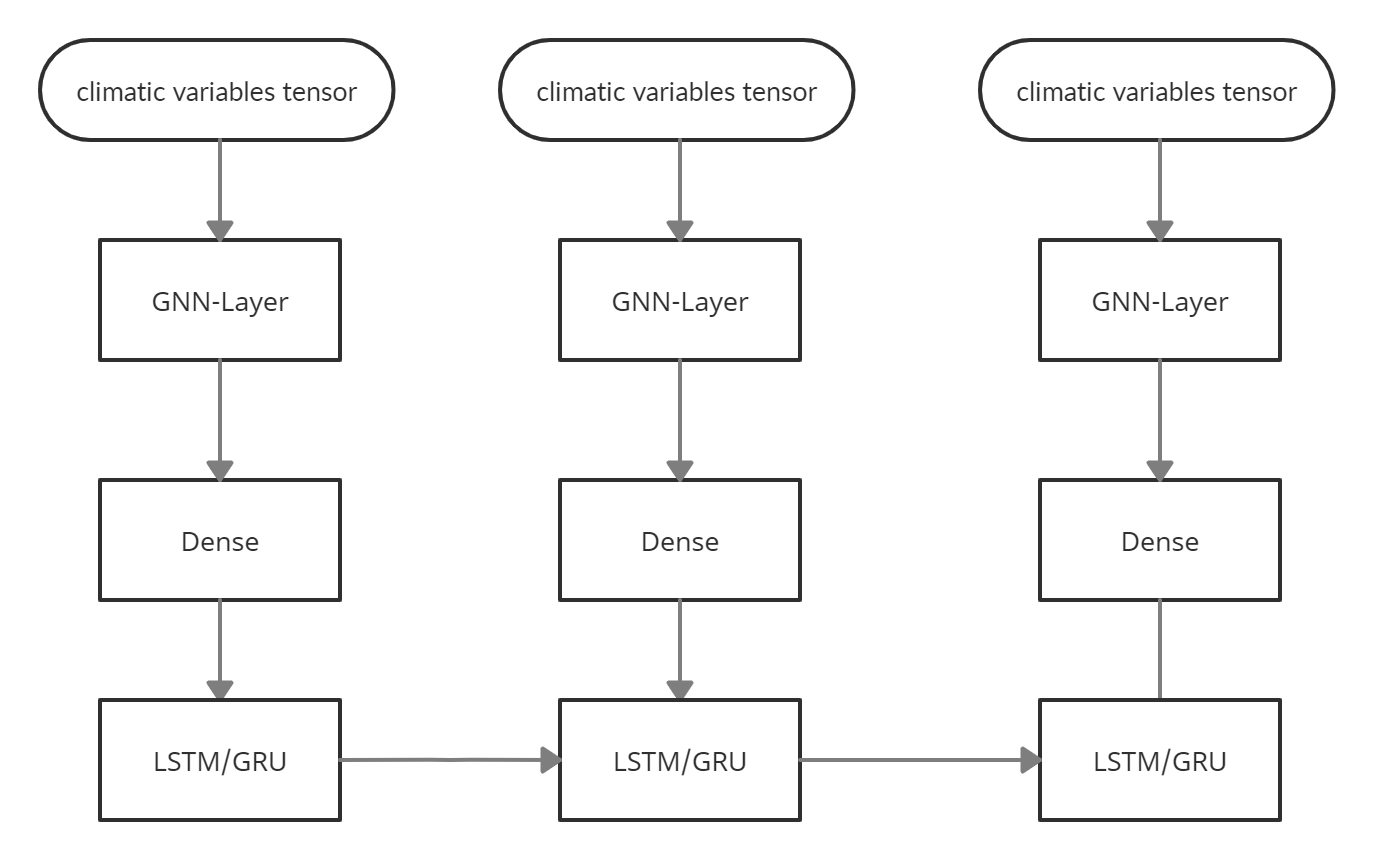
\includegraphics[scale=0.19]{figures/HailNet architecture (1).png} \\ Resulting architecture
\end{center}


\newpage
\section{Computational Experiment}
The experiment goal is to train and evaluate our model on TerraClimate and meteo.ru data.
\subsection{Data}
\subsubsection{TerraClimate}
TerraClimate is a dataset of monthly climate and climatic water balance for global terrestrial surfaces. It uses climatically aided interpolation, combining high-spatial resolution climatological normals from the WorldClim dataset, with coarser spatial resolution.

This source provides main data for the experiments. Spatial time series of various 
climatic variables. We use following variables: mean temperature above the surface, surface pressure, total precipitation, 2 components of wind.
\subsubsection{meteo.ru}
This data center provides data about hail events from 1991 year in Russia.
\subsection{Experiment Set-Up}
Unless otherwise noted, we train re-implemented \textbf{StrGNN} described in Section 2.2 and evaluate prediction accuracy, precision, recall on a test year to be predicted. The data for train and test is described in Section 3.1.

Except of training and evaluating model, the experiment goal is to optimize hyperparameters such as adjancy matrices in Graph-layers. This is important part of research, because it could be interpreted as connections between climatic values. 

Provided model is compared with SMOTE + log-regresion. This baseline is described in Section 4.

At every timestamp we have tensor of climatic variables.   
\begin{figure}[h]
\begin{minipage}[h]{0.49\linewidth}
\center{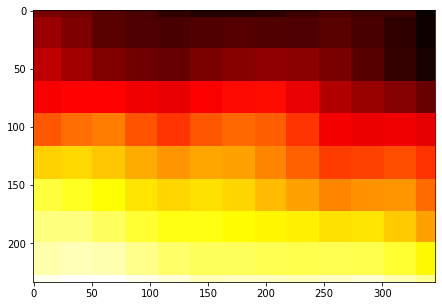
\includegraphics[scale=0.35]{figures/tmean_heat_map.png} \\ Month mean temperature}
\end{minipage}
\hfill
\begin{minipage}[h]{0.49\linewidth}
\center{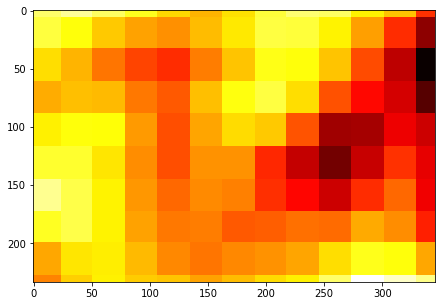
\includegraphics[scale=0.35]{figures/sp_heat_map.png} \\ Surface pressure}
\end{minipage}
\end{figure}

These variables corresponds to Tambov region.

Using GNN-layers it is possible to connect different variables and their spatial neighbourhood. It can be visualized as following: 

\begin{figure}[h]
\center{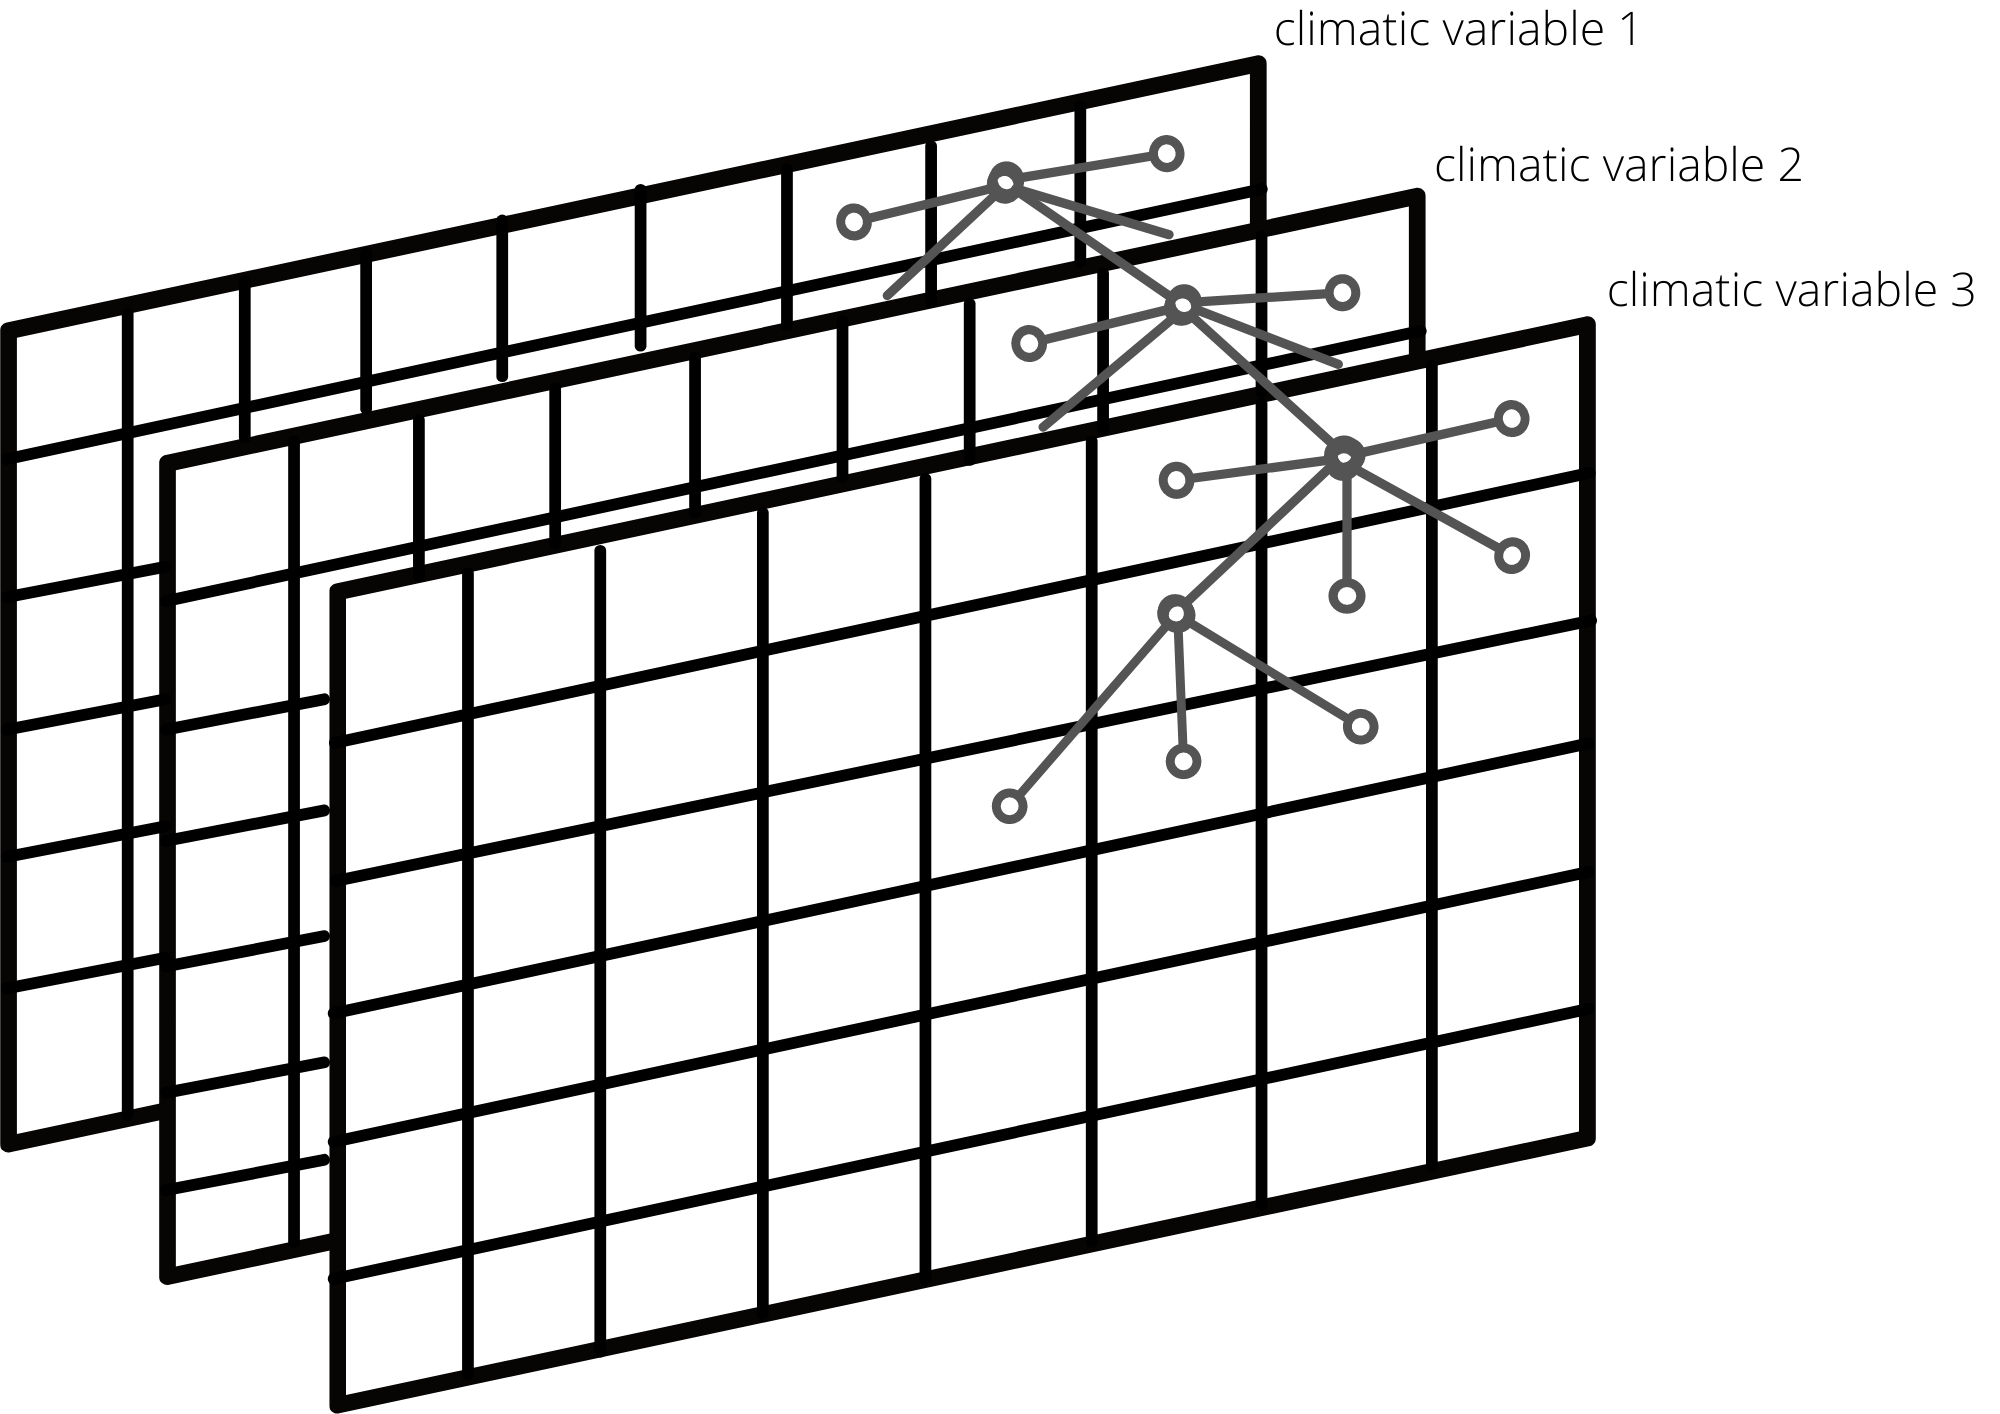
\includegraphics[scale=0.35]{figures/climate variable 1 (1).png} \\ Visualisation of principle}
\end{figure}

\newpage
Using only GNN + fully connected network we can achieve good results in classifying timestamps with hail events:
\begin{figure}[h]
\center{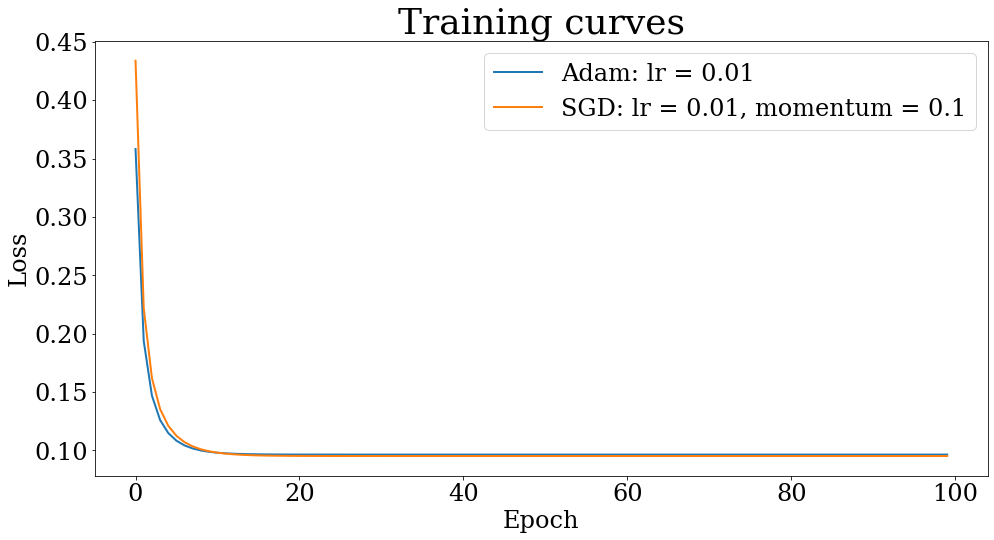
\includegraphics[scale=0.35]{figures/training_curves.png} \\}
\end{figure}

\subsection{Actual architecture}
Actual architecture is visualized as following:
\begin{figure}[h]
\center{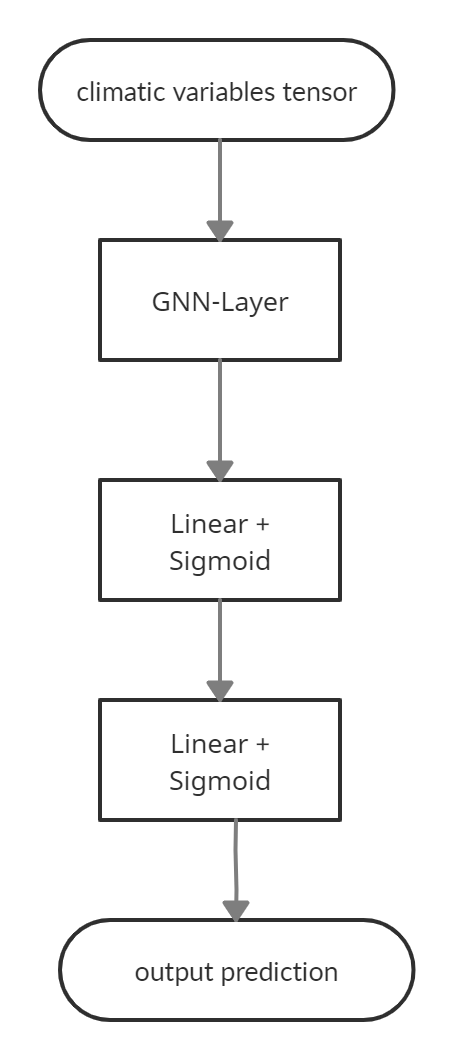
\includegraphics[scale=0.3]{figures/HailNet architecture.png} \\ HailNet architecture}
\end{figure}

\newpage
In the GNN layer we applying adjacency matrix to climatic tensor to make attention of spatial neighbourhood. After that we applying two linear layers with sigmoid activation function:
\begin{equation}
    H_1 = WAX
\end{equation}
\begin{equation}
    H_2 = \sigma(WH_1)
\end{equation}
\begin{equation}
    H_3 = \sigma(WH_2)
\end{equation}

Looking forward to modify adjacency matrix according to climate knowledge of hail events and add LSTM/GRU layers to forecast future month.


\subsection{Experiment flow}
\begin{enumerate}
    \item  Creating torch.DataLoader of downloaded climatic data from TerraClimate using Google Earth Engine and hail events data from meteo.ru.
    \item Feed 4-sized batches into training algorithm for 100 epochs.
    \item Updating HailNet parameters optimizing Binary Cross-entropy Loss with Adam optimizer and SGD optimizer.
\end{enumerate}
List of Expected tables and figures:\todo{temporary}

\begin{tabular}{c|c|c|c}
    label & precision & recall & f1 \\
    0 & 0.99 & 0.99 & 0.99 \\
    1 & 0.99 & 0.99 & 0.99
\end{tabular}

ROC-AUC plot;\\
plot of predicted probability with vspan labelling\\
\section{Preliminary report}
In order to show how does SMOTE works, there is some experiments with baseline SMOTE + logistic regression on synthetic data . Firstly, created synthetic data for classification problem with imbalanced classes in proportions $98/2$.

\begin{figure}[h]
\begin{minipage}[h]{0.49\linewidth}
\center{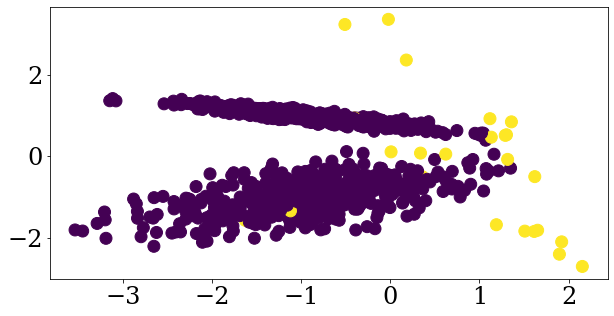
\includegraphics[scale=0.35]{synth_data_before_smote.png} \\ Data distribution before SMOTE}
\end{minipage}
\hfill
\begin{minipage}[h]{0.49\linewidth}
\center{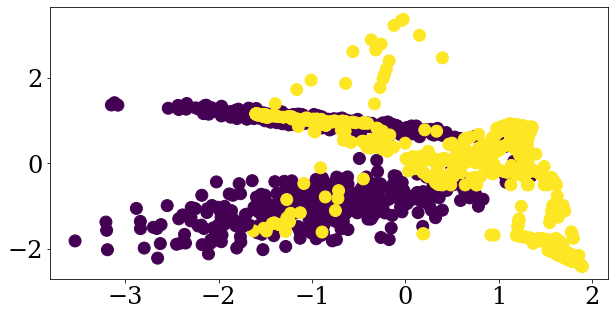
\includegraphics[scale=0.35]{synth_data_after_smote.png} \\ Data distribution after SMOTE}
\end{minipage}
\end{figure}

SMOTE works by selecting examples that are close in the feature space, drawing a line between the examples in the feature space and drawing a new sample at a point along that line. 

\begin{figure}[h]
\begin{minipage}[h]{0.49\linewidth}
\center{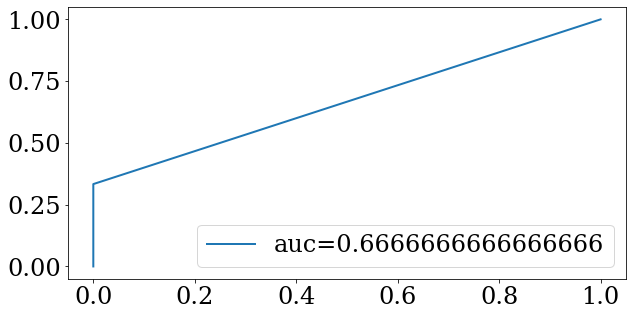
\includegraphics[scale=0.35]{auc_before_smote.png} \\ ROC-curve distribution before SMOTE}
\end{minipage}
\hfill
\begin{minipage}[h]{0.49\linewidth}
\center{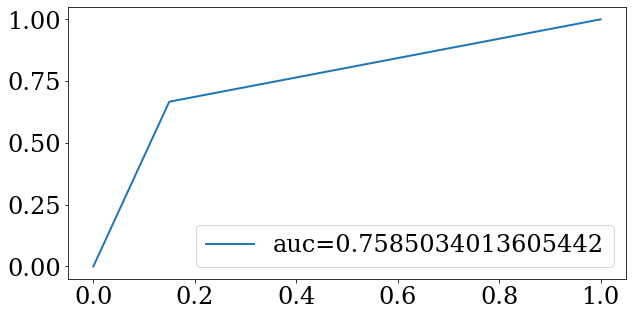
\includegraphics[scale=0.35]{auc_after_smote.png} \\ ROC-curve distribution after SMOTE}
\end{minipage}
\end{figure}

ROC-AUC increased. So we consider that SMOTE make our model better in some cases.

\section{Baselines}
The hail risk prediction is classification problems with imbalanced classes. Hail is extreme climatic event. Using SMOTE we can synthesize new examples for the minority classes \cite{DBLP:journals/corr/abs-1106-1813}. SMOTE with logistic regression is our simplest model. This model we use to compare quality with complex one. Logistic regression maps feature space into 1d probability simplex. $\mathbb{R}^n \rightarrow [0,1]$. Logistic regression model is following:
\begin{equation}
    y_i = \frac{1}{1 + e^{-x_iw}}
\end{equation}
where $x_i$ is feature vector, $w$ is parameters of the model, $y_i$ is probability of positive class labeled "1". $w$ find by LBFGS optimization algorithm minimizing log-loss function. The LBFGS optimization algorithm reviewed in details here \cite{mokhtari2014global}.
    

\bibliographystyle{abbrv}

\bibliography{references}

\end{document}